\documentclass[12pt, oneside]{article}
\usepackage{geometry}
\geometry{letterpaper, margin=1in}
\usepackage{graphicx}
\usepackage{amssymb}
\usepackage{amsmath}
\usepackage{indentfirst}
\usepackage{listings}
\usepackage{mathtools}
\usepackage{float}

\begin{document}
\section{Trajectory Geometry}

\begin{figure}[H]
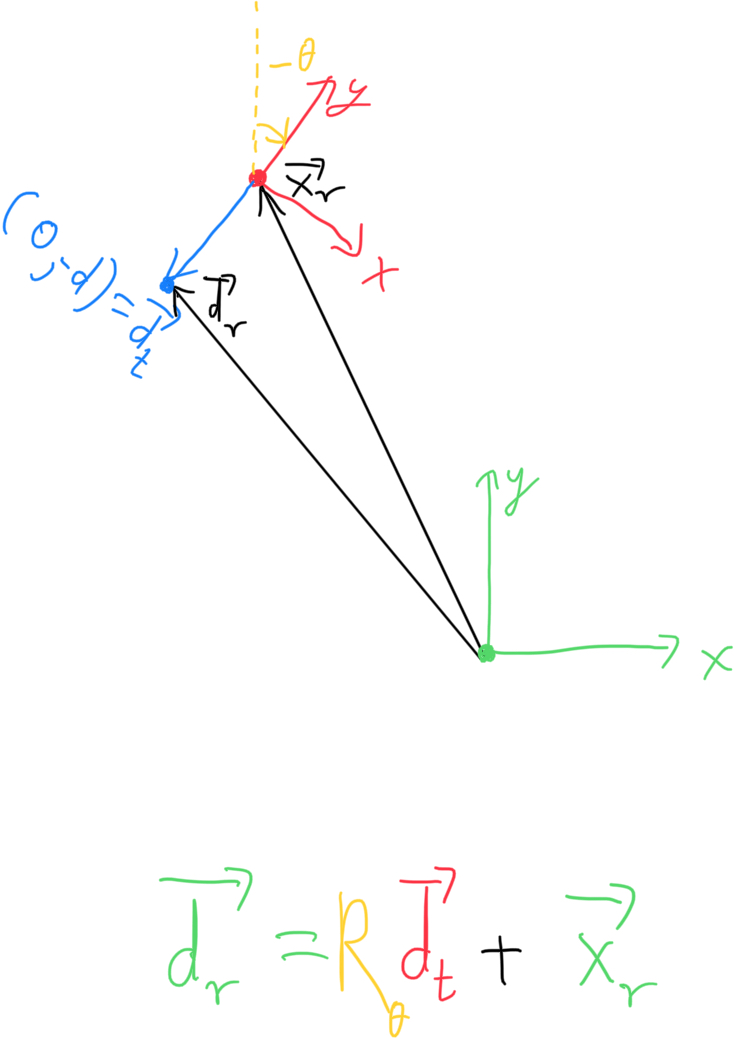
\includegraphics[width=0.5\textwidth]{Diagram.jpeg}
\centering
\end{figure}

In this diagram, the red axes represents the target's coordinate system. The green axes represent the robot's coordinate system. Points in robot's coordinate system are represented with subscript $r$, ex. $\vec{d}_r$ and points in target coordinate system are subscript $t$, so $\vec{d}_t$. 

The point we wish to navigate to is a distance $d$ in front of the target. So from the point of view of the target, the coordinate of the target point $\vec{d}_t = (0, d)$. First, we wish to find what are the coordinates of this point are from the point of view of the robot, drawn in the diagram as $\vec{d}_r$.

From CV, we know the rotation $-\theta$ of the target (and its coordinate system) relative to the robot. We also know the displacement $\vec{x}_r$ of the target's origin relative to the robot origin in robot coordinates.

Now we can construct a function $F(\vec{d}_t) \rightarrow \vec{d}_r$ that takes points in target coordinates to robot coordinates. Since points transform in the opposite direction as coordinate systems, we must apply a rotation of $+\theta$ first, then add the displacement. Therefore,

\begin{align}
\vec{d}_r &= F(\vec{d_t})\\
\vec{d}_r &= \boldsymbol{R_\theta} \vec{d_t} + \vec{x}_r\\
\vec{d_r} &= \begin{pmatrix}\cos{\theta} & -\sin{\theta}\\\sin{\theta} & \cos{\theta}\end{pmatrix} \begin{pmatrix}0 \\ -d	\end{pmatrix} + \vec{x}_r
\end{align}

Expanding this is left as an exercise for the reader. I don't remember if CV gives you the rotation of points or rotation of coordinate axes. This will flip the sign of $\theta$, but should be easy to figure out.

\end{document}